\documentclass[11pt]{article}
% Numbers: paper/check_numbers.py; provenance: paper/MANIFEST.md; figures: paper/figures.py.
% Build from paper/: `tectonic main.tex` (XeTeX), or pdflatex main && bibtex main && pdflatex main && pdflatex main.
\usepackage[margin=1in]{geometry}
\usepackage{iftex}
\ifXeTeX
  \usepackage{fontspec}  % XeTeX (e.g. Tectonic): Latin Modern via fontspec covers the accented author names in the bibliography
\else
  \usepackage[T1]{fontenc}
  \usepackage{lmodern}
\fi
\usepackage{amsmath,amssymb}
\usepackage{booktabs}
\usepackage{graphicx}
\usepackage{xcolor}
\usepackage[hidelinks]{hyperref}
\usepackage{natbib}
\usepackage{microtype}
\usepackage{adjustbox}
\usepackage{flafter}
\usepackage{listings}
\usepackage{tikz}
\usetikzlibrary{arrows.meta,positioning,calc}
\emergencystretch=2em
\renewcommand{\topfraction}{0.85}
\renewcommand{\textfraction}{0.1}
\renewcommand{\floatpagefraction}{0.75}
\setlength{\bibsep}{2pt}
\newcommand{\todo}[1]{\textcolor{red}{[TODO: #1]}}
\newcommand{\Fpre}{F_{\mathrm{pre}}}
\newcommand{\Fcore}{F_{\mathrm{core}}}
\newcommand{\Fcoda}{F_{\mathrm{coda}}}
\lstset{language=Python, basicstyle=\ttfamily\scriptsize, breaklines=true, breakatwhitespace=true, columns=fullflexible, keepspaces=true, frame=lines, framesep=4pt, xleftmargin=4pt,
  keywordstyle=\bfseries, commentstyle=\itshape\color{black!60}, showstringspaces=false}

\title{A Gated State Merge for Looped Transformer Encoders}
\author{Logan Martinez}
\date{}

\begin{document}
\maketitle

\begin{abstract}
A looped transformer applies the same layers several times, so it stores fewer parameters than a model that applies as many distinct
layers. The gated merge of \citet{zhang2026rlt}, which feeds a decoder's state from one token into the next, is adapted here to the depth
axis of a bidirectional encoder. In the encoder, a few layers are applied once, a core of layers several times, and a few final layers once; the
output of the first layers is called the anchor, and the output of the previous pass through the core the loop state. Before each pass through
the core, a correction computed from the loop state is scaled by a sigmoid gate computed from the loop state and the anchor, and is added to the
loop state. In the original merge the correction is added to the current input, whose counterpart here is the anchor. The encoders are built from ModernBERT-large layers, distilled from ModernBERT-large, and trained with the
number of passes drawn at random. In a study of four-block models with three seeds, masked-token prediction is slightly better with the merge than
without it at every number of passes from one to eight and in every seed; in a single run of an eight-block model it is better at every number of
passes. When the correction is added to the anchor instead, the model is better after one or two passes and after eight, but worse at its best
depth. The training operations, latency, and weight storage of looping are also reported.
\end{abstract}

\section{Introduction}

A looped transformer stores a small number of layers and applies them in a loop, so that its depth at inference exceeds the number of layers it
stores \citep{dehghani2019universal,lan2020albert,dabre2019recurrent,takase2021lessons}. \citet{geiping2025recurrent} split such a model into a
prelude applied once, a recurrent core applied a variable number of times, and a coda applied once. Unless something else is added, each pass
through the core starts from the previous pass's output alone.

\citet{zhang2026rlt} proposed a gated merge for a decoder that recurs across tokens. At each token, the decoder's input is the current token's
representation plus a correction computed from the previous token's final decoder state, scaled by a sigmoid gate computed from both. Here that merge is moved from the token axis to the depth axis of a bidirectional encoder: the previous token's state
becomes the loop state, the output of the previous pass through the core, and the current token's representation becomes the prelude's output,
which stays fixed across passes. The adaptation rests on three choices.
\begin{itemize}
\item The correction is added to the loop state, not to the prelude output. The prelude output is the loop's starting state, and inside the
merge it enters only through the gate.
\item The correction's projection is initialized to zero, so at the start of training the loop state is unchanged by the merge and the
model is an ordinary looped encoder.
\item The model is trained with a number of passes drawn at random at every update, so one set of weights is used at every depth from one to
eight.
\end{itemize}

All models are built from layers of ModernBERT-large \citep{warner2024modernbert} and distilled from it on masked-token prediction. The main
findings are the following.
\begin{itemize}
\item In the four-block study (three seeds), masked-token prediction with the merge is better than without it in every seed. The
distillation loss (the training objective, Section~\ref{sec:training}) on held-out text is lower by 0.0075 to 0.0136 at one, two, four, and eight passes, and the error in bits per byte defined in
Section~\ref{sec:setup} is lower at every number of passes from one to eight. The effect is small but consistent (Section~\ref{sec:merge}).
In the single eight-block run, the error in bits per byte is also lower with the merge at every number of passes (Section~\ref{sec:eight}).
\item When the correction is added to the prelude output, the counterpart of the decoder input to which it is added in the original merge,
the model is better after one or two passes and after eight, but worse at its best depth (Section~\ref{sec:merge}).
\item Counting student training only, training a looped encoder takes 2.5 to 2.6 times the floating-point operations (FLOPs) of training a
flat encoder, which applies each of the same blocks once; with the generation of the teacher's targets included, the ratio for the eight-block
models is about 1.8. At four passes the looped encoder has 1.7 to 3.0 times the flat encoder's latency on five hardware backends
(Section~\ref{sec:costs}).
\item A flat encoder that applies as many distinct blocks as a looped encoder applies in total, and so stores more parameters, predicts masked
tokens much better; it also starts from more teacher layers (Section~\ref{sec:isoflop}).
\end{itemize}

\section{Method}
\label{sec:method}

\subsection{Layout}

The encoder has eight transformer blocks: a prelude $\Fpre$ of two blocks, a core $\Fcore$ of four blocks, and a coda $\Fcoda$ of two
blocks. Let $h_0$ be the
token embeddings and $R$ the number of passes through the core. Then
\begin{equation}
a = \Fpre(h_0), \qquad x_0 = a, \qquad x_{i+1} = \Fcore\big(M(a, x_i) + s_i\big)\ \ (i = 0,\dots,R-1), \qquad y = \Fcoda(x_R).
\label{eq:layout}
\end{equation}
In words: the prelude runs once and its output $a$, called the anchor, is kept. The loop state $x$ starts equal to the anchor. In each of the $R$
passes, the anchor and the current loop state are combined by the merge $M$, a sinusoidal encoding $s_i$ of the pass number $i$ is added
\citep{vaswani2017attention,dehghani2019universal}, and the core's four blocks are applied to the result, giving the next loop state. After the last
pass the coda is applied once to the final loop state, giving the output $y$. In total $2 + 4R + 2$ blocks are applied, eight at $R = 1$ and
four more for every further pass, while only eight are stored. Without the merge, $M(a, x) = x$ and the input to the core is the previous loop state plus the pass encoding. The layout is drawn in
Figure~\ref{fig:arch}.

\begin{figure}[t]
\centering
\begin{tikzpicture}[>=Stealth, node distance=6mm,
  blk/.style={draw, rounded corners=2pt, minimum height=10mm, minimum width=19mm, align=center, font=\small},
  op/.style={draw, circle, inner sep=0.5pt, font=\small}]
\node (in) {$h_0$};
\node[blk, right=of in] (pre) {prelude $\Fpre$\\2 blocks};
\node[blk, right=13mm of pre, fill=black!6] (mrg) {merge\\$M(a, x_i)$};
\node[op, right=of mrg] (plus) {$+$};
\node[blk, right=of plus] (core) {core $\Fcore$\\4 blocks};
\node[blk, right=13mm of core] (coda) {coda $\Fcoda$\\2 blocks};
\node[right=of coda] (out) {$y$};
\node[below=6mm of plus, font=\small] (step) {$s_i$};
\draw[->] (in) -- (pre);
\draw[->] (pre) -- node[above, font=\small] {$a$} (mrg);
\draw[->] (mrg) -- (plus);
\draw[->] (step) -- (plus);
\draw[->] (plus) -- (core);
\draw[->] (core) -- node[above, font=\small] {$x_R$} (coda);
\draw[->] (coda) -- (out);
\draw[->] (core.north) -- ++(0,7mm) -| node[pos=0.25, above, font=\small] {$x_{i+1}$, for $R$ passes} (mrg.north);
\end{tikzpicture}
\caption{The looped encoder. The prelude runs once and its output $a$ (the anchor) enters the merge at every pass. The loop state $x_i$ (equal
to $a$ before the first pass) is merged with the anchor, the pass encoding $s_i$ is added, and the core is applied, giving $x_{i+1}$. After $R$ passes the
coda runs once.}
\label{fig:arch}
\end{figure}

\subsection{The merge}

\citet{zhang2026rlt} combine the representation $e_t$ of the current token $t$ with the previous token's final decoder state $z_{t-1}$ as
\begin{equation}
u_t = e_t + \alpha\, \sigma\big(W_g [e_t; r] + b_g\big) \odot W_s\, r, \qquad r = \mathrm{RMSNorm}(z_{t-1}),
\label{eq:rlt}
\end{equation}
where $[\cdot;\cdot]$ is concatenation, $\sigma$ the logistic sigmoid, $\odot$ elementwise multiplication, RMSNorm the root-mean-square
normalization of \citet{zhang2019rmsnorm}, $W_g$ and $b_g$ the weight and bias of the gate's linear layer, $W_s$ the weight of a linear
projection of the normalized state, and $\alpha$ a fixed scale. The gate $\sigma(\cdot)$ is a factor between 0 and 1 for each hidden dimension
(1024 in the models of this paper); the projected previous state is multiplied by it before it is added to the current input. The merge used here is
\begin{equation}
M(a, x) = x + \alpha\, \sigma\big(W_g [a; r] + b_g\big) \odot W_s\, r, \qquad r = \mathrm{RMSNorm}(x), \qquad \alpha = 0.1.
\label{eq:merge}
\end{equation}
The gate's inputs are of the same kind in both, the fixed representation and the normalized state; what is gated differs. In
Equation~\eqref{eq:rlt} the previous token's state enters a fresh input through the gated term, and the fresh input is the base of the sum. In
Equation~\eqref{eq:merge} the base is the loop state itself and the gated term is a correction computed from that state; the anchor appears
only as an input to the gate, so how much each dimension of the loop state is corrected depends on the anchor through the gate. The recurrence
also runs over passes through the core, with all positions of the sequence updated together, not over tokens, and the loop state starts as the
anchor instead of a learned initial state.

The projection $W_s$ is initialized to zero, so before training $M(a, x) = x$ and the model is the looped encoder without the merge
\citep{bachlechner2021rezero}; $W_g$ and $b_g$ are initialized randomly. The merge has 3.1M parameters, about 2\% of the eight-block model and 3\% of the four-block model introduced in
Section~\ref{sec:setup}.
In a variant, called the anchor residual below, the leading $x$ in Equation~\eqref{eq:merge} is replaced with $a$; the result has the form of
Equation~\eqref{eq:rlt} on the depth axis. This changes two things at once: the anchor is added in full at every pass, and the loop state no
longer passes through unchanged, entering the core only through the gated, scaled correction.

The implementation is short. The merge and the loop, from \texttt{src/arch.py} (a comment line omitted), are:
\begin{lstlisting}
def forward(self, anchor, state):
    normalized = self.norm(state)
    gate = self.gate(torch.cat((anchor, normalized), dim=-1)).sigmoid()
    return (anchor if self.base == "anchor" else state) + self.alpha * gate * self.proj(normalized)
\end{lstlisting}
\begin{lstlisting}
x = run(0, prelude, x)
a = x
for i in range(depth):
    x = run(prelude, core, (x if self.merge is None else self.merge(a, x)) + self.step(i, x))
x = run(core, self.config.num_hidden_layers, x)
\end{lstlisting}
Here \texttt{self.gate} is a linear layer with bias from $2 \times 1024$ inputs to 1024 outputs ($W_g$, $b_g$), \texttt{self.proj} a linear
layer without bias ($W_s$), \texttt{self.step} the pass encoding and \texttt{run(s, e, x)} the application of blocks $s$ to $e - 1$ to
\texttt{x}. The integers \texttt{prelude} and \texttt{core} are block indices: blocks 0 to $\texttt{prelude} - 1$ form the prelude, blocks
\texttt{prelude} to $\texttt{core} - 1$ the core and the remaining blocks the coda. The loop count \texttt{depth} is $R$, and \texttt{self.base}
is \texttt{"state"} for the merge of Equation~\eqref{eq:merge} and \texttt{"anchor"} for the anchor residual.

\subsection{Blocks and the output layer}

Every block is a ModernBERT-large layer \citep{warner2024modernbert}: pre-normalization \citep{xiong2020prelayernorm}, a GeGLU feed-forward layer
\citep{shazeer2020glu}, rotary position embeddings \citep{su2021roformer}, hidden width 1024, feed-forward width 2624, and 16 attention heads.
Each block uses either full attention or attention within a 128-token sliding window \citep{beltagy2020longformer}. In the eight-block layout,
full attention is used in the first prelude block, the first and last core blocks, and the last coda block, and sliding-window attention in the
other four. The token embeddings are copied from ModernBERT-large and
frozen, and the output layer over the vocabulary shares their weights. The prediction head before it (a dense layer and a normalization) and
the final normalization are also copied from ModernBERT-large.

\section{Training}
\label{sec:training}

\paragraph{Objective.}
In each 512-token sequence, 30\% of the positions are selected for prediction \citep{wettig2023mask,warner2024modernbert}; of these, 80\% are
replaced by the mask token, 10\% by a random token, and 10\% are left unchanged \citep{devlin2019bert}. The model being trained (the student) is
fitted to ModernBERT-large (the teacher). Let $v$ be the original token at a selected position, $p_S$ and $p_T$ the student's and the teacher's
predicted distributions there, and $p^{(\tau)}$ the distribution computed with logits divided by a temperature $\tau = 2$. With CE the
cross-entropy and KL the Kullback--Leibler divergence, the loss at the position, in the form of
\citet{hinton2015distilling} and \citet{sanh2019distilbert}, is
\begin{equation}
0.6\,\mathrm{CE}(v, p_S) + 0.4\,\tau^2\,\mathrm{KL}\big(p_T^{(\tau)} \,\big\|\, p_S^{(\tau)}\big).
\end{equation} The weights 0.6 and 0.4 were not tuned. This quantity, averaged over selected positions, is
also reported on held-out text as the \emph{distillation loss}. For each selected position the teacher's final hidden state (the input to its
output layer) is stored instead of its full distribution; applying the teacher's frozen output layer to it recovers the distribution exactly
\citep{anshumann2025sparse}. The selected positions and replacements are drawn once per sequence, when the teacher targets are produced.

\paragraph{Data.}
Training text is FineWeb sample-10BT \citep{penedo2024fineweb}, tokenized with ModernBERT's tokenizer and packed into 512-token sequences across
document boundaries \citep{liu2019roberta}. One percent of documents, selected by a hash of the document id, are held out.

\paragraph{Number of passes.}
The number of passes $R$ is drawn at every optimizer update: each group of eight consecutive updates uses every value from 1 to 8 once, in shuffled order, so every
depth is trained equally often and the mean is 4.5 passes \citep{geiping2025recurrent,huang2016stochastic}.

\paragraph{Initialization.}
Each student block starts as a copy of a teacher layer of the same attention type, chosen to be as close as possible to evenly spaced teacher
positions among its 28 layers. The merge gate is the only trained weight that is initialized randomly.

\paragraph{Optimization.}
The optimizer is AdamW \citep{loshchilov2019adamw} with learning rate $3\times10^{-4}$, weight decay 0.01, 100 warmup steps, and a cosine
schedule. Gradients are clipped at norm 1.0, computation runs in bfloat16 (bf16) autocast \citep{kalamkar2019bf16}, and each update uses 32
sequences of 512 tokens. Training uses PyTorch \citep{paszke2019pytorch} and Transformers \citep{wolf2020transformers}.

\section{Experimental setup}
\label{sec:setup}

\paragraph{Two model sizes.}
Two model sizes are used. The \emph{eight-block} models have the layout of Section~\ref{sec:method}, start from teacher layers 0, 4, 9, 11, 16, 18,
23, and 27, and are trained for 12,208 updates (200M tokens). The \emph{four-block} models halve every part: a one-block prelude, a two-block core, and a one-block coda, copied from teacher layers 0,
9, 18, and 27, all four of which use full attention; they are trained for 3,072 updates (50M tokens) from a fixed store of 98,304 teacher-labeled sequences, so every four-block run sees
identical targets. For the eight-block runs the teacher was run on a second machine, which streamed its targets to the training machine.

\paragraph{Models compared.}
At each size, three models share the same blocks and initialization: the looped encoder with the merge, the same looped encoder without the merge,
and a flat encoder that applies each stored block once, in order, with no loop, no merge, and no pass encoding. Two further models are
trained at the four-block size. The anchor-residual variant is the looped encoder with the anchor residual of Section~\ref{sec:method}. The
ten-block flat model has ten distinct blocks, copied from teacher layers 0, 2, 5, 9, 11, 14, 18, 20, 23, and 27, with full attention in every
third block as in ModernBERT. At $R = 4$ a four-block looped model applies $1 + 2\cdot 4 + 1 = 10$ blocks, as many as the ten-block flat model,
which stores more parameters. The ten-block flat model therefore has the same inference FLOPs as the looped model without the merge; the models with
the merge have about 10\% more, for the gate and projection applied at every pass. All models of
one size see the same training tokens in the same order for a given seed. They are matched in tokens, not in training compute.
The models are listed in Table~\ref{tab:arms}, with the letter used for each in the tables.

\begin{table}[t]
\centering
\small
\begin{adjustbox}{max width=\linewidth}
\begin{tabular}{llrrrrrrr}
\toprule
& & blocks & block applications & \multicolumn{2}{c}{parameters (M)} & weights & GFLOP / sequence & training \\
\cmidrule(lr){5-6}
& model & stored & at $R = 4$ & blocks + merge & total & (MB, bf16) & at $R = 4$ & tokens $\times$ seeds \\
\midrule
A & looped, merge & 8 & 20 & 101.2 & 153.9 & 308 & 264 & 200M $\times$ 1 \\
B & looped, no merge & 8 & 20 & 98.1 & 150.7 & 301 & 251 & 200M $\times$ 1 \\
C & flat & 8 & 8 & 98.1 & 150.7 & 301 & 100 & 200M $\times$ 1 \\
\midrule
A$'$ & looped, merge & 4 & 10 & 52.2 & 104.9 & 210 & 138 & 50M $\times$ 3 \\
B$'$ & looped, no merge & 4 & 10 & 49.0 & 101.7 & 203 & 125 & 50M $\times$ 3 \\
E$'$ & looped, anchor-residual merge & 4 & 10 & 52.2 & 104.9 & 210 & 138 & 50M $\times$ 3 \\
C$'$ & flat & 4 & 4 & 49.0 & 101.7 & 203 & 50 & 50M $\times$ 3 \\
D$'$ & flat, ten blocks & 10 & 10 & 122.6 & 175.3 & 351 & 125 & 50M $\times$ 3 \\
\midrule
& ModernBERT-large (teacher) & 28 & 28 & 343.2 & 395.9 & 792 & 351 & -- \\
\bottomrule
\end{tabular}
\end{adjustbox}
\caption{Models. \emph{Blocks stored}: distinct transformer blocks held in memory. \emph{Block applications}: blocks applied in one forward
pass at $R = 4$ (prelude + $4\times$ core + coda for looped models). \emph{Parameters, blocks + merge}: the parameters that differ between
models, each stored block counted once. \emph{Parameters, total}: also includes the 51.6M-parameter token embedding table (frozen, copied from the
teacher and shared with the output layer) and the 1.1M-parameter prediction head. \emph{Weights}: total parameters at two bytes each, which is
weight storage, not peak memory. \emph{GFLOP}: operations of one forward pass of the encoder (without the output layer) on one 512-token
sequence, as counted by PyTorch's FLOP counter; what that count includes and omits is described in Section~\ref{sec:costs}.}
\label{tab:arms}
\end{table}

\paragraph{Seeds.}
The four-block models were trained with three seeds each. Because every block starts as a copy of a teacher layer, only the merge gate's
initialization, the order of the training data, and the sequence of sampled depths differ between seeds; the spread over seeds is therefore not a spread over
independently initialized weights. The eight-block models were trained once each. One eight-block looped run is counted at 359 PFLOP ($10^{15}$ floating-point
operations, counted as described in Section~\ref{sec:costs}) of training, 7.2 times a four-block looped run. It occupied the training GPU for
3.2 hours (with the merge) or 2.8 hours (without), with the teacher machine running for the same time. Repeated seeds were therefore run at the
four-block size, where the fifteen runs (five models, three seeds each) together cost fewer operations than the three eight-block runs, whether or
not the teacher's work is included.

\paragraph{Metric.}
\label{sec:metric}
An encoder that sees context on both sides of a token does not assign a probability to a whole text, so the perplexity used for left-to-right
language models is not available. The main metric is instead the error on the task the models are trained on, predicting masked tokens from
their context, on held-out text from several domains. For each text, the tokens (at most 512, special tokens excluded) are split into eight
interleaved groups, token $j$ going to group $j \bmod 8$. In each of eight forward passes one group is replaced by the mask token, so every
token is predicted exactly once while seven eighths of the text is visible. The score is the sum, over tokens, of $-\log_2$ of the probability assigned
to the true token in the pass that masks it, divided by the number of UTF-8 bytes of text those tokens cover. This is partition-masked bits
per byte (PM-BPB); lower is better. With the sum divided by bytes instead of tokens, models with different tokenizers are on one scale, although what a mask
hides still depends on the tokenizer, so only comparisons among the students, which share one tokenizer, are controlled. PM-BPB differs from the
pseudo-log-likelihood of \citet{salazar2020mlmscoring}, which masks one token at a time.

The held-out text has four sources of 128 texts each, every text the first 1,000 characters of a document: the FineWeb hold-out, arXiv articles
\citep{cohan2018arxiv}, English Wikipedia \citep{wikimedia2023wikipedia}, and Python code \citep{codeparrot2022clean}. Losses and byte counts
are summed within a source, and the reported mean is the unweighted mean of the four sources. Per-text scores were not kept, so the uncertainty
reported for PM-BPB is the spread over seeds, not over texts.

\paragraph{Comparison depth.}
Looped models are compared at $R = 4$. That depth was fixed after the four-block results were known, as the depth at which the four-block
looped models with and without the merge scored best, so it is not an independent choice. Results at every depth are shown in the figures.

\paragraph{Reference encoders.}
RoBERTa-base \citep{liu2019roberta}, DeBERTa-base \citep{he2021deberta}, DistilBERT-base-cased \citep{sanh2019distilbert}, and the teacher are
scored the same way. They differ from the students in tokenizer, training data, and objective, so their scores give a familiar scale and are not
controlled comparisons.

\section{Results}
\label{sec:results}

\subsection{The merge and the anchor residual}
\label{sec:merge}

PM-BPB of the four-block models at every depth, and the differences between models trained with the same seed, are plotted in
Figure~\ref{fig:four}. All three looped models improve steeply up to $R = 3$. With the merge,
PM-BPB at $R = 4$ is 0.928, against 0.931 without it; both rise again toward $R = 8$ (0.949 and 0.953). With the anchor residual, PM-BPB is
lower than with the merge at $R = 1$ (1.007, against 1.054 with the merge) and at $R = 2$ (0.955 against 0.957), and higher from $R = 3$ to 7
(0.947 against 0.934 at $R = 3$). From $R = 4$ on it stays at 0.943, while the merged model's PM-BPB rises to 0.949 at $R = 8$, so at $R = 8$ the
anchor residual is lower than the merge again. Its value at its best depth, 0.943, is above the merged model's best, 0.928. The flat
model with the same four blocks has PM-BPB 0.978.

\begin{figure}[!tbp]
\centering
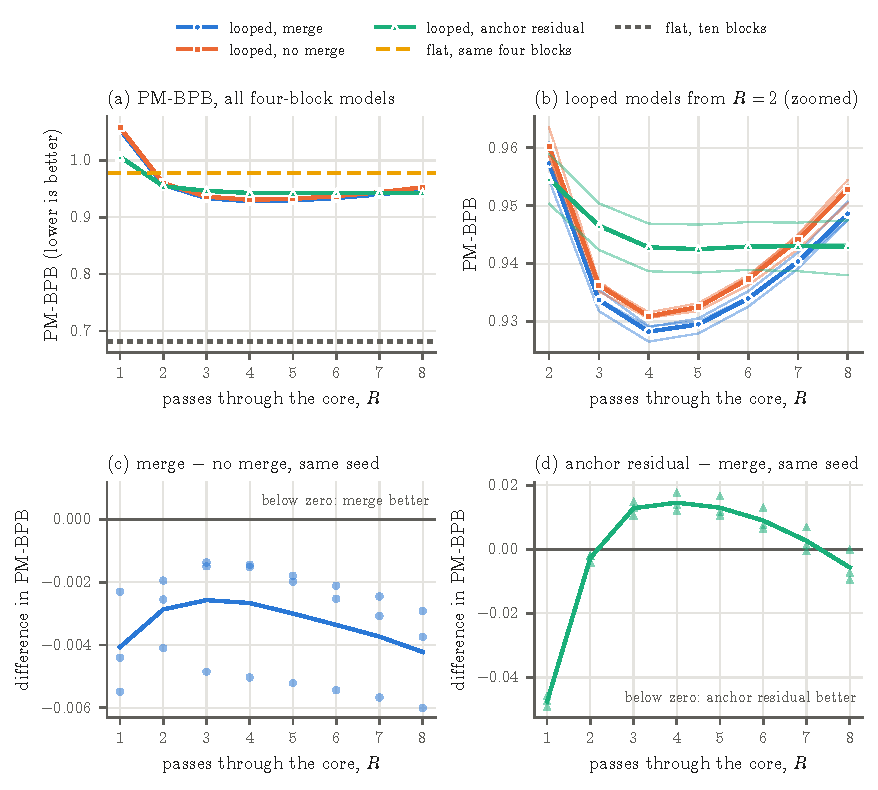
\includegraphics[width=\linewidth]{figures/pmbpb_four_block.pdf}
\caption{Four-block models after 50M tokens; each panel has its own vertical scale. (a) PM-BPB against the number of passes $R$, mean over
three seeds, with the two flat models as horizontal lines. (b) The looped models from $R = 2$ on, with each seed as a thin line. (c, d) Differences
in PM-BPB between models trained with the same seed (points: seeds; line: mean); below zero, the first-named model is better.}
\label{fig:four}
\end{figure}

Because models trained with the same seed see the same data in the same order and, if looped, the same sequence of depths, differences within a
seed are not affected by those two sources of variation. The random initialization of the merge gate, which only the models with a merge have,
still varies with the seed and is part of each difference. They are listed in Table~\ref{tab:paired}. Each entry is the first model's score minus the second's; for both
measures, lower is better.

\begin{table}[t]
\centering
\small
\begin{tabular}{llrrrr}
\toprule
comparison & measure & seed 1 & seed 2 & seed 3 & mean \\
\midrule
merge (A$'$ $-$ B$'$) & loss, $R = 1$ & $-0.0116$ & $-0.0119$ & $-0.0111$ & $-0.0115$ \\
merge (A$'$ $-$ B$'$) & loss, $R = 2$ & $-0.0078$ & $-0.0083$ & $-0.0101$ & $-0.0087$ \\
merge (A$'$ $-$ B$'$) & loss, $R = 4$ & $-0.0075$ & $-0.0084$ & $-0.0108$ & $-0.0089$ \\
merge (A$'$ $-$ B$'$) & loss, $R = 8$ & $-0.0097$ & $-0.0106$ & $-0.0136$ & $-0.0113$ \\
merge (A$'$ $-$ B$'$) & PM-BPB, $R = 4$ & $-0.0014$ & $-0.0015$ & $-0.0050$ & $-0.0027$ \\
anchor residual (E$'$ $-$ A$'$) & PM-BPB, $R = 4$ & $+0.0177$ & $+0.0138$ & $+0.0121$ & $+0.0146$ \\
looping (B$'$ $-$ C$'$) & PM-BPB, $R = 4$ & $-0.0499$ & $-0.0476$ & $-0.0431$ & $-0.0469$ \\
\bottomrule
\end{tabular}
\caption{Differences between four-block models trained with the same seed. \emph{Loss}: held-out FineWeb distillation loss. \emph{PM-BPB}: mean
over the four sources.}
\label{tab:paired}
\end{table}

With the merge, the held-out distillation loss is lower than without it in every seed at each of the four depths at which it was recorded,
by 0.0075 to 0.0136. PM-BPB is lower in every seed at every depth from 1 to 8 (Figure~\ref{fig:four}c), by 0.0014 to 0.0060; at $R = 4$
the difference is 0.0014 to 0.0050. Per source, it is lower with the merge in all 24 depth--seed pairs on FineWeb, arXiv, and Wikipedia, and in
14 of 24 on code. The two models differ by the whole merge, including its 3.1M parameters and 10\% more FLOPs at $R = 4$, so
the gain cannot be attributed to the gate, to the anchor input, or to the extra parameters separately.

The anchor residual is worse than the merge at $R = 4$ in every seed, by 0.012 to 0.018 PM-BPB. Its held-out distillation loss is lower at $R = 1$ (3.274
against 3.434 with the merge) and higher at $R = 4$ (2.981 against 2.925). From $R = 4$ to $R = 8$ its distillation loss still falls slightly in
every seed, while that of both other looped models rises. Both changes described in Section~\ref{sec:method} are made in the anchor residual, and which of them is
responsible cannot be determined from these results.

With the same four blocks looped instead of applied once, PM-BPB is lower by 0.043 to 0.050, at about 2.5 times the student-training operations
(Section~\ref{sec:costs}). This is consistent with earlier work on looped models \citep{lan2020albert,dehghani2019universal}.

\subsection{Eight-block models}
\label{sec:eight}

PM-BPB per source for the eight-block models is listed in Table~\ref{tab:main}, and the mean at every depth is plotted in
Figure~\ref{fig:eight}. The pattern of the four-block study holds with one seed: with the merge, PM-BPB is lower than without it at every depth from 1 to 8,
by 0.0006 to 0.0041 (0.613 against 0.616 at $R = 4$; Figure~\ref{fig:eight}b), and both looped models have
lower PM-BPB than the flat model (0.655) on every source. In PM-BPB both looped models are best at $R = 4$, the merged model equally at $R = 5$, and lose 0.008
(with the merge) and 0.009 (without) by $R = 8$. The held-out FineWeb distillation loss at $R = 4$ is 1.947 with the merge, 1.955 without, and
2.162 for the flat model; in that loss both looped models are best at $R = 6$ (1.935 and 1.944). At $R = 1$ the looped models are worse than the flat model (0.708 against 0.655), although they then apply the same eight
blocks; they were trained across all depths and carry the pass encoding, while the flat model was trained only for its single depth.

Per source, the merge's advantage in the eight-block models is largest on code, 0.0050 to 0.0092 at every depth. On FineWeb the merged model is
better or equal at every depth. On arXiv and Wikipedia it is slightly worse at the lower depths, by at most 0.0016, and better at every depth from
$R = 5$ on. With one seed, these per-source differences carry no estimate of their spread.

\begin{table}[t]
\centering
\small
\begin{adjustbox}{max width=\linewidth}
\begin{tabular}{llrrrrr}
\toprule
model & $R$ & FineWeb & arXiv & Wikipedia & code & mean \\
\midrule
A looped, merge & 1 & 0.615 & 0.767 & 0.586 & 0.863 & 0.708 \\
A looped, merge & 4 & \textbf{0.526} & \textbf{0.667} & \textbf{0.514} & \textbf{0.746} & \textbf{0.613} \\
A looped, merge & 8 & 0.527 & 0.672 & 0.517 & 0.768 & 0.621 \\
B looped, no merge & 1 & 0.615 & 0.765 & 0.585 & 0.868 & 0.708 \\
B looped, no merge & 4 & 0.527 & 0.668 & \textbf{0.514} & 0.755 & 0.616 \\
B looped, no merge & 8 & 0.529 & 0.676 & 0.518 & 0.776 & 0.625 \\
C flat & -- & 0.566 & 0.715 & 0.543 & 0.795 & 0.655 \\
\midrule
ModernBERT-large (teacher) & -- & 0.315 & 0.326 & 0.281 & 0.191 & 0.278 \\
RoBERTa-base & -- & 0.618 & 0.732 & 0.665 & 1.644 & 0.915 \\
DeBERTa-base & -- & 0.673 & 0.777 & 0.722 & 1.521 & 0.923 \\
DistilBERT-base-cased & -- & 0.991 & 0.681 & 0.768 & 1.625 & 1.016 \\
\bottomrule
\end{tabular}
\end{adjustbox}
\caption{PM-BPB (lower is better) of the eight-block models after 200M tokens, one seed each, and of four reference encoders. Bold: the lowest value in each column among the
students. Reference encoders use other tokenizers, data, and objectives. With the 512-token limit, the scores of RoBERTa-base and DeBERTa-base on code cover 0.5\% fewer bytes
than the students'.}
\label{tab:main}
\end{table}

\begin{figure}[!tbp]
\centering
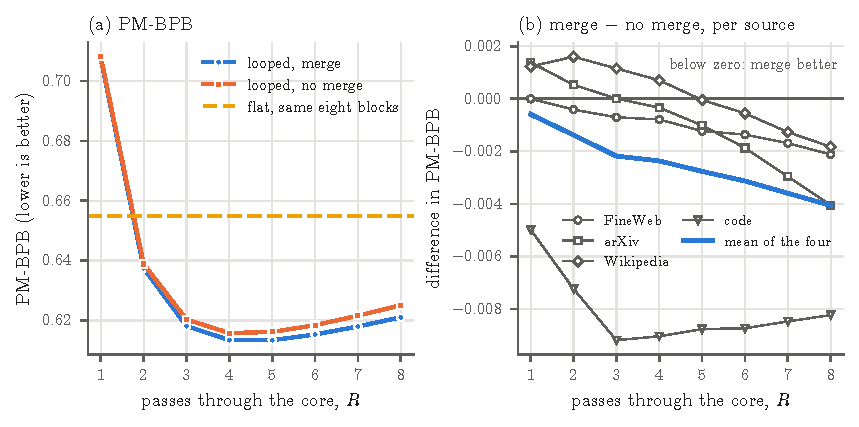
\includegraphics[width=\linewidth]{figures/pmbpb_eight_block.pdf}
\caption{Eight-block models after 200M tokens, one seed each. (a) PM-BPB against the number of passes $R$; the dashed line is the flat model
with the same eight blocks. (b) PM-BPB with the merge minus without it, for each source and for their mean; below zero, the merged model is
better.}
\label{fig:eight}
\end{figure}

With one exception, the flat model against DistilBERT-base-cased on arXiv, all three eight-block students (the looped ones at $R = 4$) have
lower PM-BPB than RoBERTa-base, DeBERTa-base, and DistilBERT-base-cased on every source, with the largest gap on code. The students inherit the teacher's tokenizer, its embeddings, and layers trained
on data that include code, so this gap is not evidence about the architecture.

\subsection{Equal inference FLOPs}
\label{sec:isoflop}

The comparison is made with the four-block looped model without the merge, which at $R = 4$ has exactly the inference FLOPs of the ten-block
flat model (125 GFLOP per sequence, Table~\ref{tab:arms}). The ten-block flat model has PM-BPB 0.681, against 0.931 for the looped model,
with 1.7 times its total parameters and 2.5 times its block parameters. At equal inference FLOPs, distinct
blocks are much better than repeated ones here; what looping saves is parameters. The ten-block model also starts from ten teacher layers instead
of four, so in this comparison looping is not separated from the larger initialization.

\subsection{Costs}
\label{sec:costs}

\paragraph{Training compute.}
Training compute was obtained with PyTorch's FLOP counter (module \texttt{flop\_counter}) on one distillation step, forward and backward,
for one 512-token sequence, including the decoding of the stored teacher state. Only matrix multiplications and attention are counted;
normalizations, activation functions, the gate's sigmoid, and other elementwise operations are not counted, nor are the optimizer and data loading. A
sliding-window block is counted like a full-attention block (attention over all 512 positions), because the window is applied as a mask; the
counted attention work of the sliding-window blocks is therefore larger than the work the window requires. For the looped models, steps at $R = 1$
and $R = 2$ were counted and the cost at $R = 3$ to 8 was extended linearly, since every pass applies the same blocks to a tensor of the same
size. The teacher's forward pass was counted on copies with one and two layers and scaled to its 28 layers. The no-merge models were assigned the
merged models' count, which overstates them by the merge's share.

On this basis, one 200M-token run is counted at 359 PFLOP for an eight-block looped model and 137 for the flat model, a ratio of 2.63
computed from the unrounded counts; for the four-block models the ratio is 2.54. These ratios count student training only. The teacher targets
for 200M tokens are counted at another 137 PFLOP, which is assigned to each eight-block run here, although the looped run with the merge and the
flat run shared one teacher pass. With the teacher targets included in this way, the eight-block ratio is 1.81. The four-block models all read
one store of teacher targets, built once, so no such ratio is given for them. A flat model given as many training operations as
a looped one would need 2.63 times the tokens and, with the same accounting, 2.63 times the teacher targets, about 721 PFLOP against 497 for a
looped run. Matching the students' training operations and matching the whole pipeline's operations therefore give different baselines
\citep{kaplan2020scaling,hoffmann2022chinchilla}.

\paragraph{Latency.}
The timed workload is one masked-language-model forward pass on one 512-token sequence, with output logits computed at 30\% of the positions.
Each configuration was run three times as warm-up and then timed call by call for at least 3 seconds and at least eight calls; the median is reported in
Table~\ref{tab:latency}. Five backends were measured. The first is an NVIDIA RTX 5070 under PyTorch 2.11.0 \citep{paszke2019pytorch} in eager mode with bf16
weights. The other four use an Intel Core Ultra 7 265K: its neural processing unit (NPU) and integrated GPU (iGPU) through OpenVINO 2026.4.1
\citep{openvino} in fp16 (16-bit floating point), and its CPU through OpenVINO and through PyTorch, both in fp32 (32-bit floating point). Every model was timed at $R = 4$ on every backend in one pass per backend (the anchor-residual variant in a later
pass of its own). An earlier sweep, in a different session, timed the same configurations where it covered them; its values are within 3\% of
the table's on the NPU, 4\% on the integrated GPU, 9\% on the RTX 5070, 17\% on the PyTorch CPU path, and 21\% on the OpenVINO CPU path, so
smaller differences between sessions are not meaningful. On the PyTorch CPU path the four-block looped models at $R = 4$ also switched between
two modes from run to run, near 155 and near 199 ms.

\begin{table}[t]
\centering
\small
\begin{adjustbox}{max width=\linewidth}
\begin{tabular}{llrrrrr}
\toprule
& & RTX 5070 & Intel NPU & Intel iGPU & Intel CPU & Intel CPU \\
& model & PyTorch, bf16 & OpenVINO, fp16 & OpenVINO, fp16 & OpenVINO, fp32 & PyTorch, fp32 \\
\midrule
A & looped, merge, $R = 4$ & 13.7 & 195.4 & 183.3 & 354.9 & 276.7 \\
B & looped, no merge, $R = 4$ & 12.8 & 166.8 & 184.0 & 346.8 & 262.6 \\
C & flat & 5.5 & 71.5 & 92.9 & 153.4 & 121.9 \\
\midrule
A$'$ & looped, merge, $R = 4$ & 7.7 & 127.2 & 109.7 & 198.6 & 159.7 \\
B$'$ & looped, no merge, $R = 4$ & 6.9 & 87.6 & 105.5 & 186.4 & 136.7 \\
E$'$ & looped, anchor residual, $R = 4$ & 7.9 & 125.8 & 108.5 & 193.1 & 167.8 \\
C$'$ & flat & 3.0 & 42.6 & 62.6 & 83.1 & 63.9 \\
D$'$ & flat, ten blocks & 6.6 & 84.9 & 108.2 & 185.2 & 141.5 \\
\midrule
& ModernBERT-large (teacher) & 16.7 & 205.4 & 245.8 & 464.9 & 370.3 \\
\bottomrule
\end{tabular}
\end{adjustbox}
\caption{Median latency (ms) of one masked-LM forward pass on one 512-token sequence, batch size 1, every cell measured, the looped models at
$R = 4$. Four-block models: seed-1 checkpoints; the eight-block models have one seed. The variation between sessions is given in the text.}
\label{tab:latency}
\end{table}

On every backend the looped models at $R = 4$ are slower than the flat models with the same blocks, by 1.7 times (four blocks without the
merge, integrated GPU) to 3.0 times (four blocks with the merge, NPU). The merge itself adds latency: on the NPU by 45\% for the four-block models
and 17\% for the eight-block models, and on the other backends by at most 17\%. The ten-block flat model applies as many blocks as the
four-block looped models at $R = 4$ and has the same counted inference FLOPs as the one without the merge; its latency is within 4\% of the
four-block looped model without the merge on every backend. The anchor-residual variant, with the same FLOP count as the merged model, is within
5\% of the merged model's latency on every backend.

\paragraph{Memory.}
At inference, the activations of one pass through the core are released before the next pass, so activation memory does not grow with $R$. It
depends on the width and the sequence length, which all students share, and on the runtime. Weight storage is therefore the memory quantity that
differs between the models, and peak memory was not measured. Weight storage is listed in Table~\ref{tab:arms}; it is 308 MB in bf16 for
the eight-block looped model with the merge and 792 MB for the teacher. During training, the activations of all $R$ passes are kept for back-propagation, so training memory does grow with $R$; it was not measured either.

\paragraph{Weight quantization.}
The weights of every linear layer inside the blocks were rounded to symmetric integers, per output channel for int8 and in groups of 64 input
features for int4, and the models were evaluated with the rounded weights converted back to bf16. The embeddings, prediction head, output layer,
and merge stayed in bf16, and no calibration data was used. The result is a measure of sensitivity to rounding, not of the speed or memory of low-bit kernels. The
four-block models were evaluated at their seed-1 checkpoints. With int8 weights, the mean PM-BPB of every evaluated student, at either size,
changes by less than 0.0012. With int4 weights
it rises by 0.025 to 0.03 for the eight-block models, looped and flat alike; among the four-block models by 0.038 for the flat model, 0.045 for
the looped models with and without the merge at $R \le 4$ (0.06 at $R = 8$), and 0.025 for the anchor-residual variant. For RoBERTa-base, quantized
the same way, it rises by 0.115.

\subsection{Halting}
\label{sec:halting}

A looped model can in principle stop early on easy inputs \citep{graves2016act}. To estimate how much a stopping rule could save, the distillation
loss of every looped model with and without the merge (not the anchor-residual variant) was recorded at every depth from 1 to 8 for 512 held-out FineWeb and 512 arXiv sequences, together with the loop state
averaged over each sequence's selected positions. Under a stopping rule, each sequence is assigned a depth and the recorded loss at that depth;
the rule's \emph{budget} is the mean number of passes over sequences. The savings are therefore computed from recorded losses, not from timed runs. Each
rule is compared with a fixed depth at the same budget, interpolated linearly between the two neighboring depths, and its \emph{gain} is the
reduction in loss against that fixed depth, for budgets between 2.5 and 7.5 passes. As an upper reference, under an oracle rule each sequence is given the depth that minimizes its
recorded loss plus a price per pass, with 60 prices.

The stopping rule tested is a single logistic regression, shared by all depths, whose input is the averaged loop state after a pass. It
was fitted on the states of 4,096 separate training sequences at every depth to predict whether the loss at that depth is within 0.02 of the
sequence's lowest loss over all eight depths; the stopping depth is the first depth at which the predicted probability
exceeds a threshold. Over 30 thresholds, the best gain is 0.0001 to 0.0025 across models and sources (with the threshold chosen on the evaluated sequences,
so optimistic). The gain averaged over the thresholds whose budgets lie between 2.5 and 7.5 passes is $-0.0087$ to $+0.0004$ across models and
sources. At the thresholds 0.3, 0.5, 0.7, and 0.9, whose budgets and gains are reported separately and
not limited to 2.5 to 7.5 passes, budgets span 3.9 to 7.9 passes and gains are at most 0.0012. The oracle's best gain is 0.014 to 0.018. In an earlier exploration on the
eight-block merged model, other training targets were tried (stopping when no later depth is better, or regressing the improvement still to
come), as were other features (depth, and the change and confidence of the output distribution) and heads with one hidden layer of 256 units.
That exploration used its own sequences: 10,240 for training and 512 held-out FineWeb and 512 held-out arXiv sequences, different from those
above. On them the best gains were at most 0.0046 with linear heads and 0.0063 with hidden layers, against oracle gains of 0.0149 on FineWeb and
0.0213 on arXiv. Little of the oracle's gain is recovered by the rules tested.

\subsection{Zero-shot natural language inference}
\label{sec:nli}

Three tasks of the General Language Understanding Evaluation benchmark (GLUE) were used \citep{wang2019glue}: Multi-Genre Natural Language
Inference (MNLI, \citealp{williams2018mnli}), Question Natural Language Inference (QNLI, built from \citealp{rajpurkar2016squad}), and Recognizing
Textual Entailment (RTE, \citealp{dagan2006rte}). Each example of their development sets was written as a cloze prompt in each of two
templates: ``\emph{first} ? [MASK] , \emph{second}'' and ``\emph{first} Question: \emph{second} ? Answer: [MASK] .'', where [MASK] is the
mask token, \emph{first} the premise and \emph{second} the hypothesis; for QNLI, the question comes first and the sentence second. The predicted label is the label word
with the highest log-probability at the mask \citep{schick2021pet,gao2021lmbff}; the label words are ``Yes'', ``Maybe'', and ``No'' for MNLI and
``Yes'' and ``No'' for QNLI and RTE. Each label word's score is calibrated by subtracting its log-probability on a content-free prompt, in which
both sentences are ``N/A'' \citep{zhao2021calibrate}. Accuracy is averaged over the two templates and reported with calibration and, in
parentheses, without it. No model was trained on any benchmark. On QNLI and RTE every model, the teacher included, stays
within about 2.5 standard errors of always predicting the most frequent class (50.5\% and 52.7\%). On MNLI, where that rate is 35.3\%, the
teacher reaches 41.8\% (43.6\%). The ten-block flat model reaches 38.4\% (40.6\%), about three points above the majority rate, while the
four-block looped models at $R = 4$ and the four-block flat model are at 34.3 to 35.3\% with and without calibration. The eight-block looped
models at $R = 4$ and the eight-block flat model are at 33.7 to 35.8\% with calibration and 38.4 to 41.4\% without, so their gain over the
majority rate does not remain after calibration. Only the ten-block flat model is above the majority rate with calibration, and the models
with and without the merge are not distinguished by this test.

\section{Related work}
\label{sec:related}

\paragraph{Looped and depth-recurrent transformers.}
The Universal Transformer applies one block repeatedly with a per-step encoding and adaptive halting \citep{dehghani2019universal}. Repeating
layers compressed BERT \citep{lan2020albert} and translation models \citep{dabre2019recurrent,takase2021lessons}. Looped transformers can express
iterative algorithms \citep{giannou2023looped} and learn them sample-efficiently \citep{yang2024looped}, and can approach deeper models on reasoning tasks
\citep{saunshi2025latent}. \citet{geiping2025recurrent} train a decoder with a prelude, a
recurrent core, and a coda on a random number of iterations, injecting the prelude output at every iteration. In MoEUT, mixture-of-experts
layers are added to a looped model \citep{csordas2024moeut}, and Relaxed Recursive Transformers initialize a looped model from a pretrained flat one
\citep{bae2025relaxed}.

\paragraph{Feedback and gated residuals.}
\citet{zhang2026rlt} and feedback transformers \citep{fan2020feedback} pass later states back to earlier computation along the sequence. Gated
residual updates appear in highway networks \citep{srivastava2015highway} and the gated Transformer-XL \citep{parisotto2020gtrxl}, and
zero-initialized residual branches start as the identity \citep{bachlechner2021rezero}. Depth-recurrent and implicit models usually inject the
input at every iteration \citep{bai2019deq,geiping2025recurrent,yang2024looped}, as the anchor residual does.

\paragraph{Encoder distillation.}
DistilBERT, PKD, TinyBERT, and MiniLM distill BERT-style encoders \citep{sanh2019distilbert,sun2019pkd,jiao2020tinybert,wang2020minilm} with the
soft-target loss of \citet{hinton2015distilling}. When only the top teacher logits are cached, the stored distribution is
biased \citep{anshumann2025sparse}; with the teacher's final hidden state stored instead, that bias is avoided.

\paragraph{Adaptive depth.}
Per-token halting \citep{graves2016act,banino2021pondernet,elbayad2020depthadaptive,bae2025mor}, confidence-based exits \citep{schuster2022calm},
and early exit in BERT \citep{xin2020deebert,zhou2020pabee} spend fewer layers on easy inputs.

\section{Limitations}

All evidence is masked-token prediction; no model was fine-tuned for classification or retrieval, so transfer to downstream tasks is untested.
The models are matched in training tokens, and no flat model was trained with the looped models' training operations. The merge was compared
only with no merge and with the anchor residual, so its gain is not divided among the gate, the anchor input, and the added parameters. The
eight-block results rest on one run per model, and the FLOP-matched flat model exists only at the four-block size. Quantization was simulated.
Both model sizes are small and every student is distilled from one teacher; the results may differ at larger scale, with longer training, or
without distillation.

\section{Conclusion}

With the gated merge of \citet{zhang2026rlt} moved from the token axis to the depth axis of a looped encoder, the best results in these
experiments come from adding the gated correction to the loop state rather than to the prelude output. In that form, masked-token prediction in
the four-block study is slightly better with the merge than without it at every depth and in every seed, and in the single eight-block run it is
better at every depth. In the anchor-residual form, the counterpart of the original merge, the model is better than with the merge after one or
two passes and after eight, but worse at its best depth (0.943 against 0.928 PM-BPB). Counting student training only, training a looped encoder
takes 2.5 to 2.6 times the operations of training a flat model with the same stored blocks; with the teacher's targets included, the eight-block
ratio is about 1.8. At four passes the looped encoder's latency is 1.7 to 3.0 times as high on five hardware backends. At equal counted
inference FLOPs in the four-block comparison, looping saved weight storage (203 MB for the looped model without the merge, against 351 MB for
the ten-block flat model), while the ten-block flat model had a substantially lower PM-BPB (0.681 against 0.931); it also starts from more
teacher layers.

\section*{Code and data availability}

Code, the result files, a script that checks the paper's numbers against the result files, and a reproduction script that runs every
training and evaluation step are available at \url{https://github.com/lmartinezai/rltforencoder}; no trained models are released. The reproduction script's
training commands were checked field by field against the arguments that each of the 18 trained models stored with itself. Library versions: PyTorch 2.11.0 \citep{paszke2019pytorch}, Transformers 5.22.2 \citep{wolf2020transformers}, OpenVINO 2026.4.1
\citep{openvino}. Data and
teacher revisions: FineWeb \texttt{9bb295dd}, ModernBERT-large \texttt{45bb4654}, arxiv-summarization \texttt{240aaf1a}, Wikipedia 20231101.en
\texttt{b04c8d1c}, codeparrot-clean-valid \texttt{4db92d2e}, GLUE \texttt{bcdcba79}. The three eight-block runs record identical hashes of the
teacher target stream and of the evaluation set. The whole project, including earlier exploratory runs, is counted at 2.65 EFLOP ($10^{18}$ operations)
under the accounting of Section~\ref{sec:costs}, with a 2\% allowance for evaluation during training and approximate counts for the earliest runs.
This total excludes the evaluations reported here.

\bibliographystyle{plainnat}
\bibliography{../references}

\end{document}
